\iffalse
\chapter{Software Development}
\label{chap:software-development}

\section{Software Development Methodology}
\label{section:software-development-methodology}
<TIP: Describe your software development methodology in this section. />

\section{Technology Stack}
\label{section:technology-stack}
<TIP: Describe your technology stack here. See the following example from ThaiProgrammer.org />
\begin{figure}[h]
    \centering
    \includegraphics[width=0.5\textwidth]{examples/tech-stack.png}
    \caption{Example technology stack}
\end{figure}

\section{Coding Standards}
\label{section:coding-standards}
<TIP: Describe your coding standard for this project here. />
\fi
\section{Schedule}
\label{section:schedule}

Table ~\ref{tab:schedule} presents the project schedule organized into
five phases across a 14-week development period.

\begin{table}[h]
    \centering
    \renewcommand{\arraystretch}{1.4}
    \caption{Project Schedule}
    \label{tab:schedule}
    \begin{tabular}{|l|l|p{7cm}|}
        \hline
        \textbf{Phase} & \textbf{Weeks} & \textbf{Tasks} \\
        \hline
        Planning \& Setup
            & Weeks 1--2
            & Study the problem domain and prepare development tools
              and environment. \\
        \hline
        Data Preparation
            & Weeks 3--5
            & Collect, label, and organize video data. \\
        \hline
        Feature Extraction
            & Weeks 6--8
            & Extract pose keypoints using MediaPipe and convert
              outputs to time-series data for model input. \\
        \hline
        Model Development
            & Weeks 9--11
            & Test the YOLO and MediaPipe integration, train the
              LSTM classifier (Axel vs Non-Axel), and evaluate
              model performance. \\
        \hline
        Extension \& Finalization
            & Weeks 12--14
            & Extend classification to Toe vs Edge and multi-class
              scenarios, then build the demo and prepare the
              final presentation. \\
        \hline
    \end{tabular}
\end{table}

Figure ~\ref{fig:gantt} illustrates the same schedule as a Gantt chart,
showing the timeline and overlap between phases.

\begin{figure}[h]
    \centering
    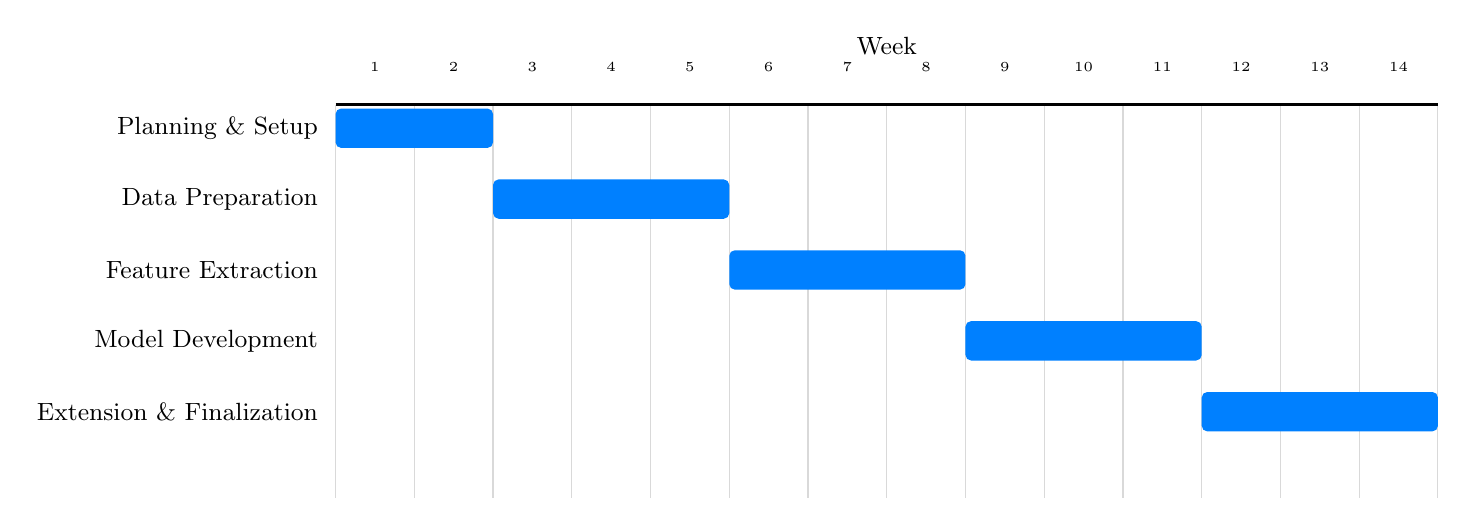
\begin{tikzpicture}
        \def\totalweeks{14}
        \def\barheight{0.5}
        \def\rowgap{0.9}

        % Phase definitions: {label}{start}{duration}
        \def\phases{
            {Planning \& Setup}{1}{2},
            {Data Preparation}{3}{3},
            {Feature Extraction}{6}{3},
            {Model Development}{9}{3},
            {Extension \& Finalization}{12}{3}
        }

        % Week axis labels
        \foreach \w in {1,...,14} {
            \node[font=\tiny, anchor=south] at (\w - 0.5, 0.1) {\w};
        }
        \node[font=\small, anchor=west] at (0, 0.5) {};

        % Grid lines
        \foreach \w in {1,...,15} {
            \draw[gray!30, thin] (\w - 1, -0.2) -- (\w - 1, -5.2);
        }

        % Bars
        \foreach \i/\label/\start/\dur in {
            0/Planning \& Setup/1/2,
            1/Data Preparation/3/3,
            2/Feature Extraction/6/3,
            3/Model Development/9/3,
            4/Extension \& Finalization/12/3
        } {
            \pgfmathsetmacro\ypos{-\i * \rowgap - 0.5}
            % Bar
            \fill[blue!50!cyan, rounded corners=2pt]
                (\start - 1, \ypos - \barheight/2)
                rectangle
                (\start + \dur - 1, \ypos + \barheight/2);
            % Label on left
            \node[font=\small, anchor=east] at (-0.1, \ypos) {\label};
        }

        % Bottom axis line
        \draw[thick] (0, -0.2) -- (14, -0.2);

        % Week label
        \node[font=\small] at (7, 0.55) {Week};
    \end{tikzpicture}
    \caption{Gantt Chart of Project Schedule}
    \label{fig:gantt}
\end{figure}

\section{Progress Tracking Report}
\label{section:progress-tracking-report}